\cmfnewsection{Modelo em Referencial Síncrono}{./logos/fundo_tese}{0.15}







%%%%%%%%%%%%%%%%%%%%%%%%%%%%%%%%%%%%%%%%%%%%%%%%%%%%%%%
%%%%%%%%%%%%%%%%%%%%%%%%%%%%%%%%%%%%%%%%%%%%%%%%%%%%%%%
%%%%%%%%%%%%%%%%%%%%%%%%%%%%%%%%%%%%%%%%%%%%%%%%%%%%%%%
\begin{frame}{Sistema de Controle em Referencial Síncrono}




\begin{columns}
\column{0.7\textwidth}
\centering

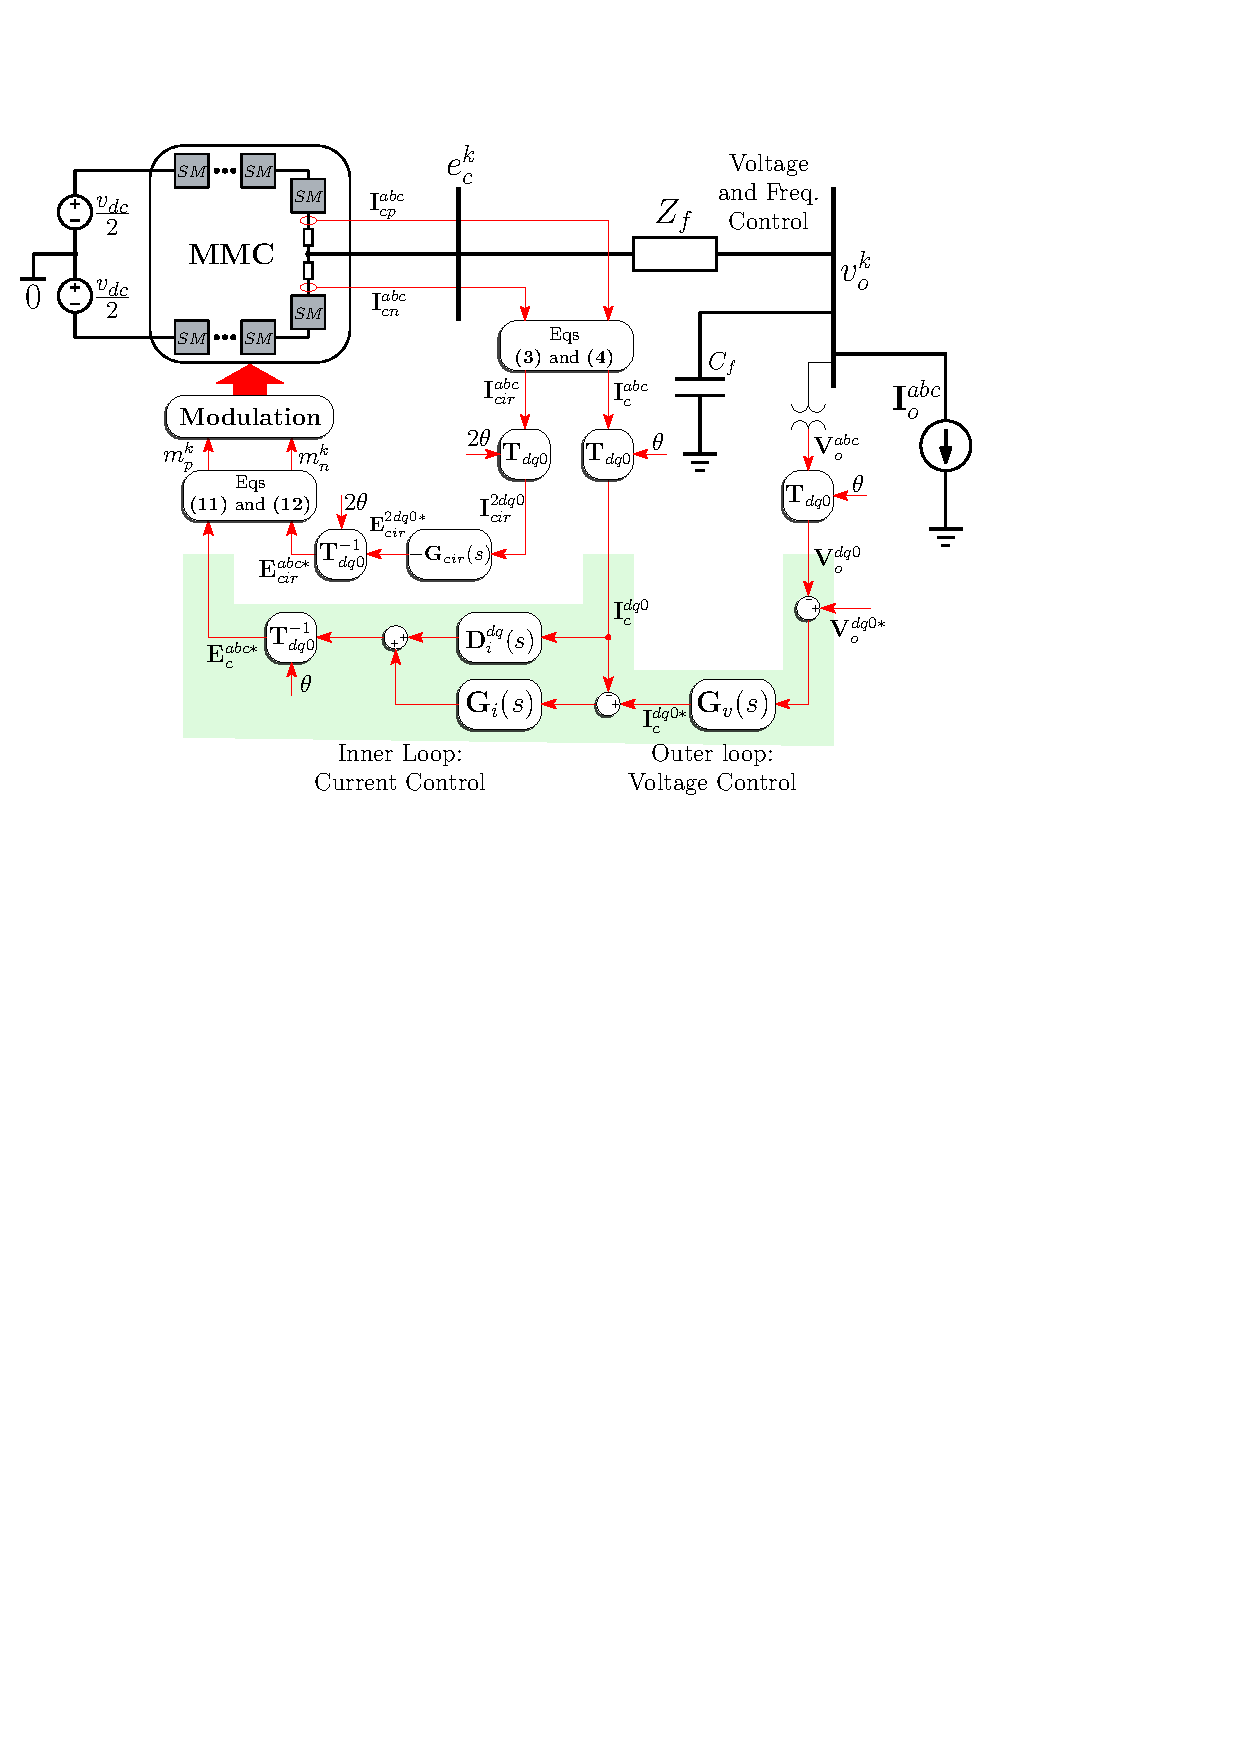
\includegraphics[width=0.95\linewidth]{./figuras/figuras_srf/controle_VI_SRF2}

\column{0.3\textwidth}
\centering

Controladores

\begin{equation*}
G_{cir}(s) = k_p^{icir} + \frac{k_i^{icir} }{s}
\end{equation*}

\begin{equation*}
G_i(s) = k_p^i + \frac{k_i^i}{s}
\end{equation*} 

%\begin{equation*}
%\decidq = \frac{L +2L_f}{V_{dc0}}\vetowcoupling
%\end{equation*} 

\begin{equation*}
G_{v,sl}(s) = k_p^{v,dl} + \frac{k_i^{v,dl}}{s}
\end{equation*} 

\end{columns}


\end{frame}




%
%%%%%%%%%%%%%%%%%%%%%%%%%%%%%%%%%%%%%%%%%%%%%%%%%%%%%%%%
%%%%%%%%%%%%%%%%%%%%%%%%%%%%%%%%%%%%%%%%%%%%%%%%%%%%%%%%
%%%%%%%%%%%%%%%%%%%%%%%%%%%%%%%%%%%%%%%%%%%%%%%%%%%%%%%%
%\begin{frame}{Transformação de Park}
%
%\centering
%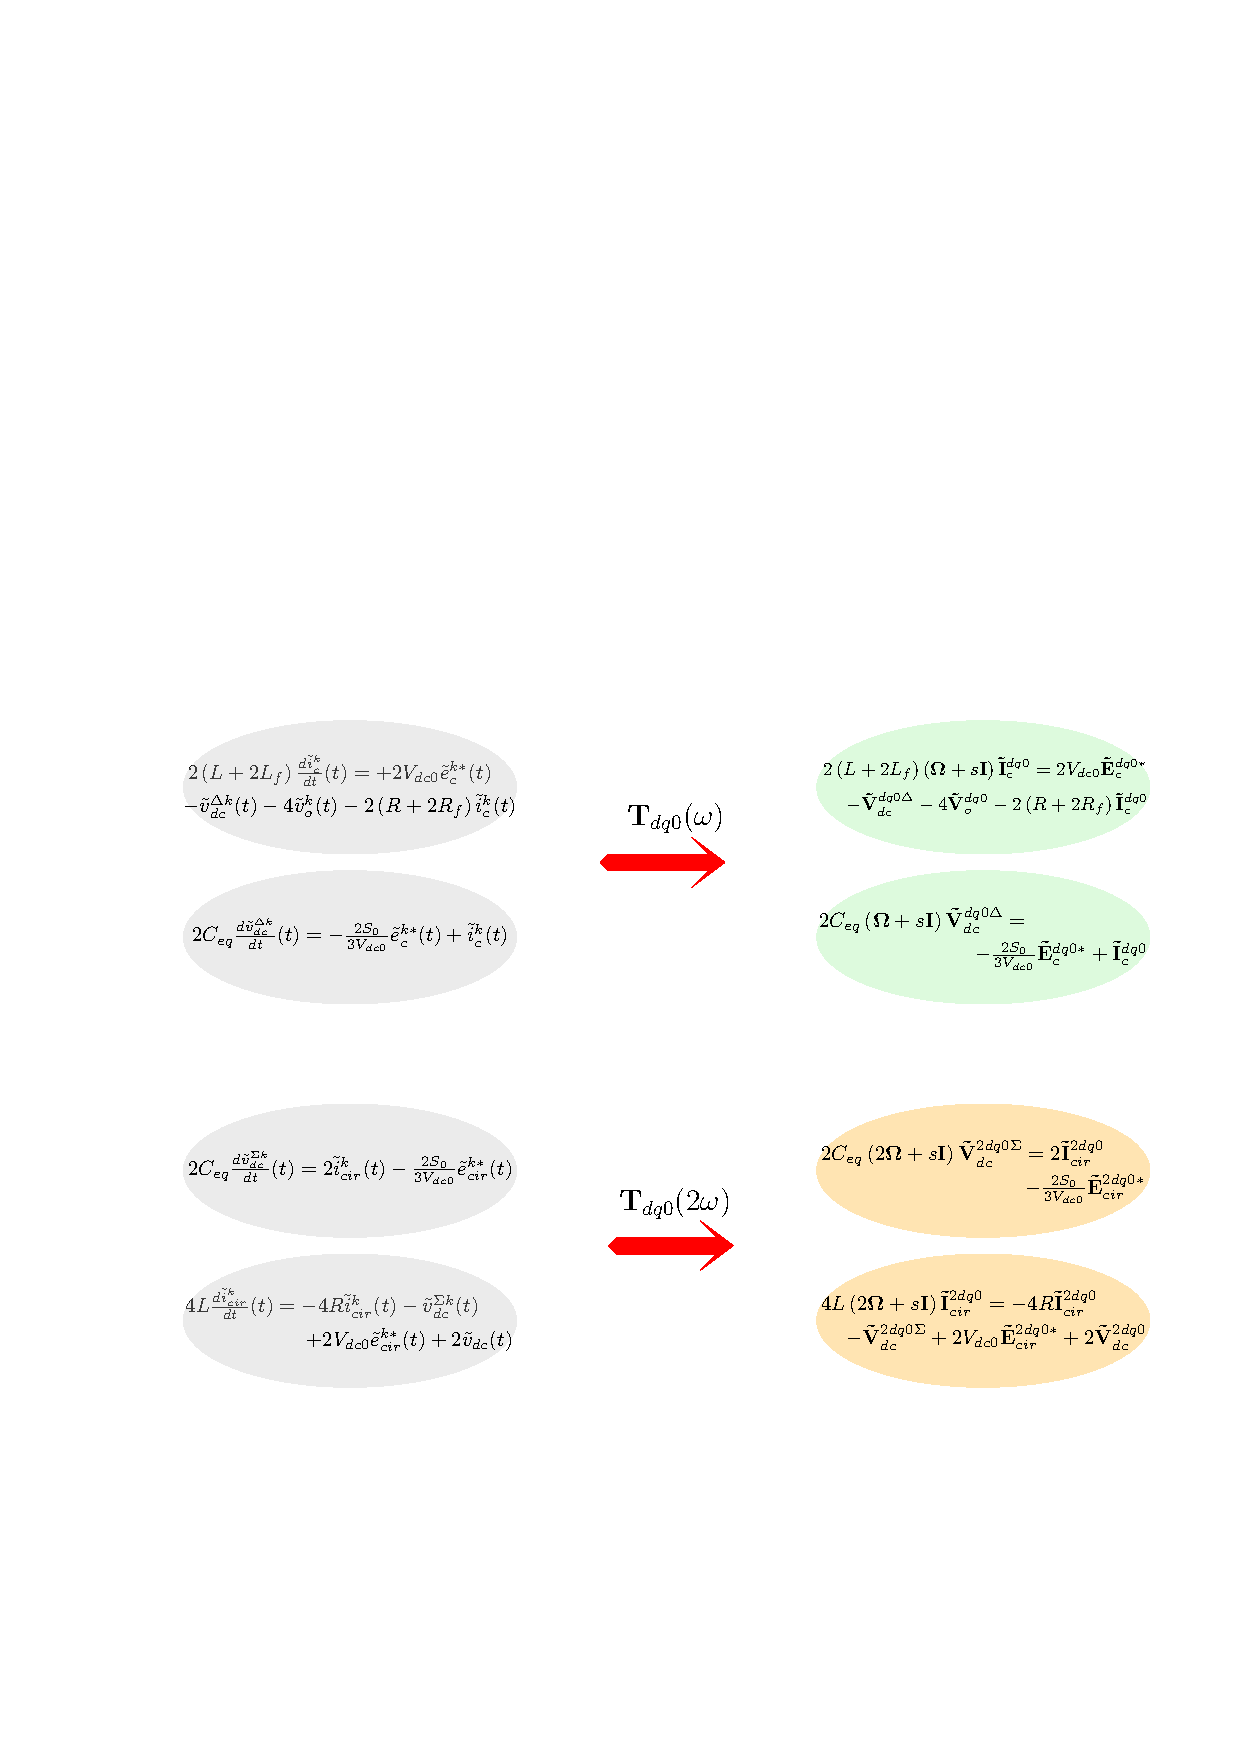
\includegraphics[width=0.7\linewidth]{./figuras/figuras_srf/park}
%
%\end{frame}
%


%%%%%%%%%%%%%%%%%%%%%%%%%%%%%%%%%%%%%%%%%%%%%%%%%%%%%%%
%%%%%%%%%%%%%%%%%%%%%%%%%%%%%%%%%%%%%%%%%%%%%%%%%%%%%%%
%%%%%%%%%%%%%%%%%%%%%%%%%%%%%%%%%%%%%%%%%%%%%%%%%%%%%%%
\begin{frame}{Transformação de Park}
\setbeamercolor{block title}{bg=gray!30,fg=black}

\centering
\begin{block}{Referencial Natural}


\begin{equation*}
 2\left( L + 2 L_f \right)  \frac{d \tilde{i}_c^k}{dt}(t) =   
 2V_{dc0}\tilde{e}_c^{k*}(t)
  -
  \tilde{v}_{dc}^{\Delta k}(t)  
 - 4 \tilde{v}_o^k(t) 
- 2\left(R + 2 R_f \right) \tilde{i}_c^k(t)
\end{equation*}

\begin{equation*}
2 C_{eq}  \frac{d \tilde{v}_{dc}^{\Delta k}}{dt}(t) = 
- \frac{2 S_0}{3 V_{dc0}} \tilde{e}_c^{k*}(t) 
+ \tilde{i}_c^{k}(t)
\end{equation*}

\end{block}



\begin{block}{Referencial Síncrono}

\begin{equation*}
 2\left( L + 2 L_f \right) \left( \vetowcoupling  
+  s \mathbf{I} \right)\vetoricdqL= 
   2V_{dc0} \vetorecdqL
   -  \vetorvdcdeltadqL  
 - 4 \vetorvodqL 
- 2\left(R + 2 R_f \right) \vetoricdqL
\end{equation*}

\begin{equation*}
2 C_{eq} \left( \vetowcoupling  
+  s \mathbf{I} \right) \vetorvdcdeltadqL  =
-\frac{2 S_0}{3 V_{dc0}} \vetorecdqL 
+ \vetoricdqL
\end{equation*}


\end{block}

\end{frame}





%%%%%%%%%%%%%%%%%%%%%%%%%%%%%%%%%%%%%%%%%%%%%%%%%%%%%%%
%%%%%%%%%%%%%%%%%%%%%%%%%%%%%%%%%%%%%%%%%%%%%%%%%%%%%%%
%%%%%%%%%%%%%%%%%%%%%%%%%%%%%%%%%%%%%%%%%%%%%%%%%%%%%%%
\begin{frame}{Modelo da Malha de Corrente}


%\begin{itemize}
%	\item Corresponde a malha que fecha através de $G_i(s)$
%	
%	\item Representa a malha interna do MMC sob controle de malha dupla	
%	
%\end{itemize}
%
%\vspace*{1.0cm}

\begin{columns}

\column{0.4\textwidth}
\centering

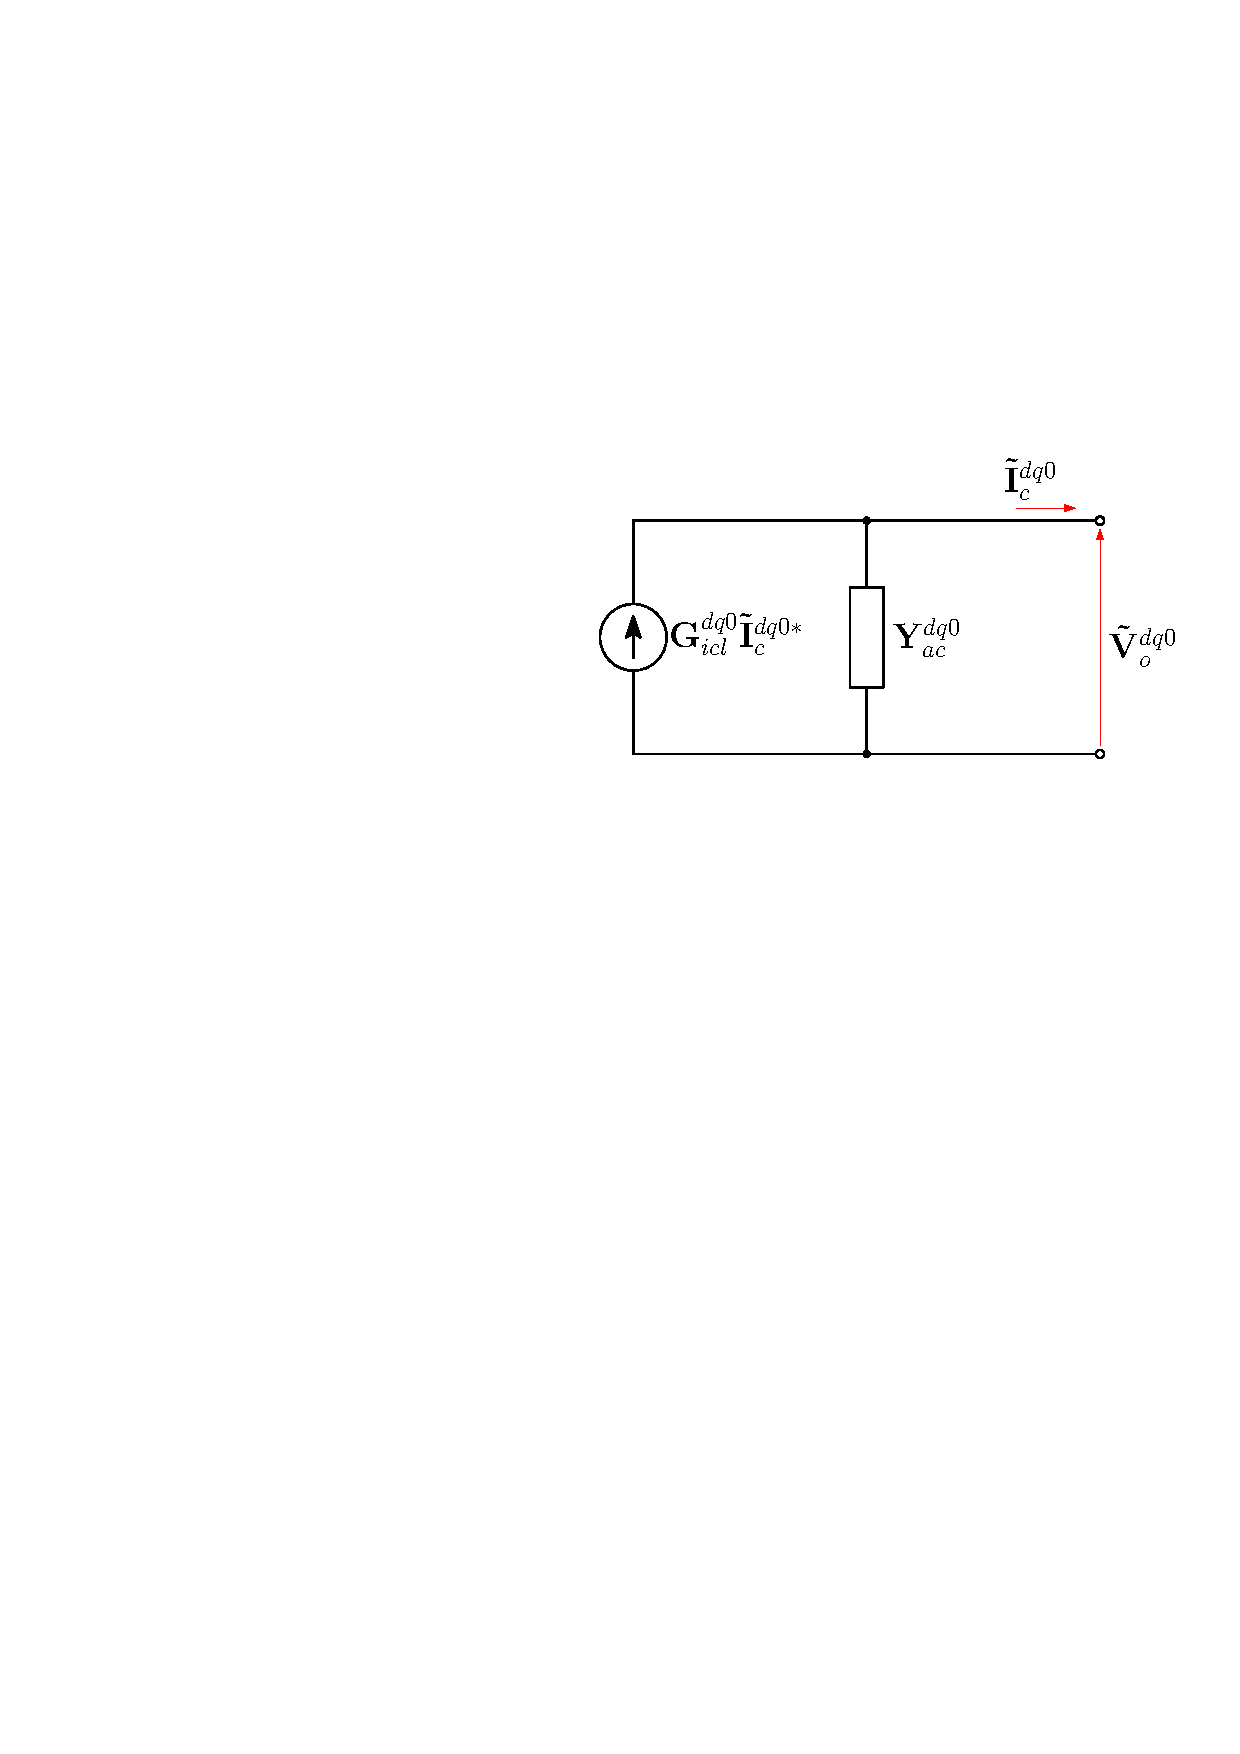
\includegraphics[width=0.9\linewidth]{./figuras/figuras_srf/Northon_SRF_I}


\column{0.6\textwidth}
\centering

\begin{itemize}
	\item Ganho e admitâncias são matrizes $3 \times 3$\\[5pt] 
	\item A admitância é influenciada pelos parâmetros de controle
\end{itemize}



\end{columns}

\vspace*{0.5cm}



\begin{equation*}
\vetoryacdqL(s) = 8 C_{eq} \vetorgichardqL^{-1}(s)\sdq
\end{equation*}
%
%
%
\begin{equation*}
%\resizebox{0.9\textwidth}{!} 
%{$
\vetorgicldqL(s) = \vetorgichardqL^{-1}(s) \left(4 C_{eq} V_{dc0} \sdq  +\frac{2 S_0}{3 V_{dc0}} \mathbf{I}\right)\vetorgidq(s)
%$}
\end{equation*}
%
\begin{equation*}
\vetorgichardqL(s) = 
\mathbf{I} +
\left(4 C_{eq} V_{dc0} \sdq  +\frac{2 S_0}{3 V_{dc0}} \mathbf{I}\right) \vetorgidq(s)
+ 4 C_{eq}  \left( Z + 2Z_f \right) \sdq
 - \frac{2 S_0}{3 V_{dc0}} \decidq
\end{equation*} 

\end{frame}






%%%%%%%%%%%%%%%%%%%%%%%%%%%%%%%%%%%%%%%%%%%%%%%%%%%%%%%
%%%%%%%%%%%%%%%%%%%%%%%%%%%%%%%%%%%%%%%%%%%%%%%%%%%%%%%
%%%%%%%%%%%%%%%%%%%%%%%%%%%%%%%%%%%%%%%%%%%%%%%%%%%%%%%
\begin{frame}{Modelo da Malha de Tensão}




\begin{columns}

\column{0.4\textwidth}
\centering

\vspace*{0.5cm}

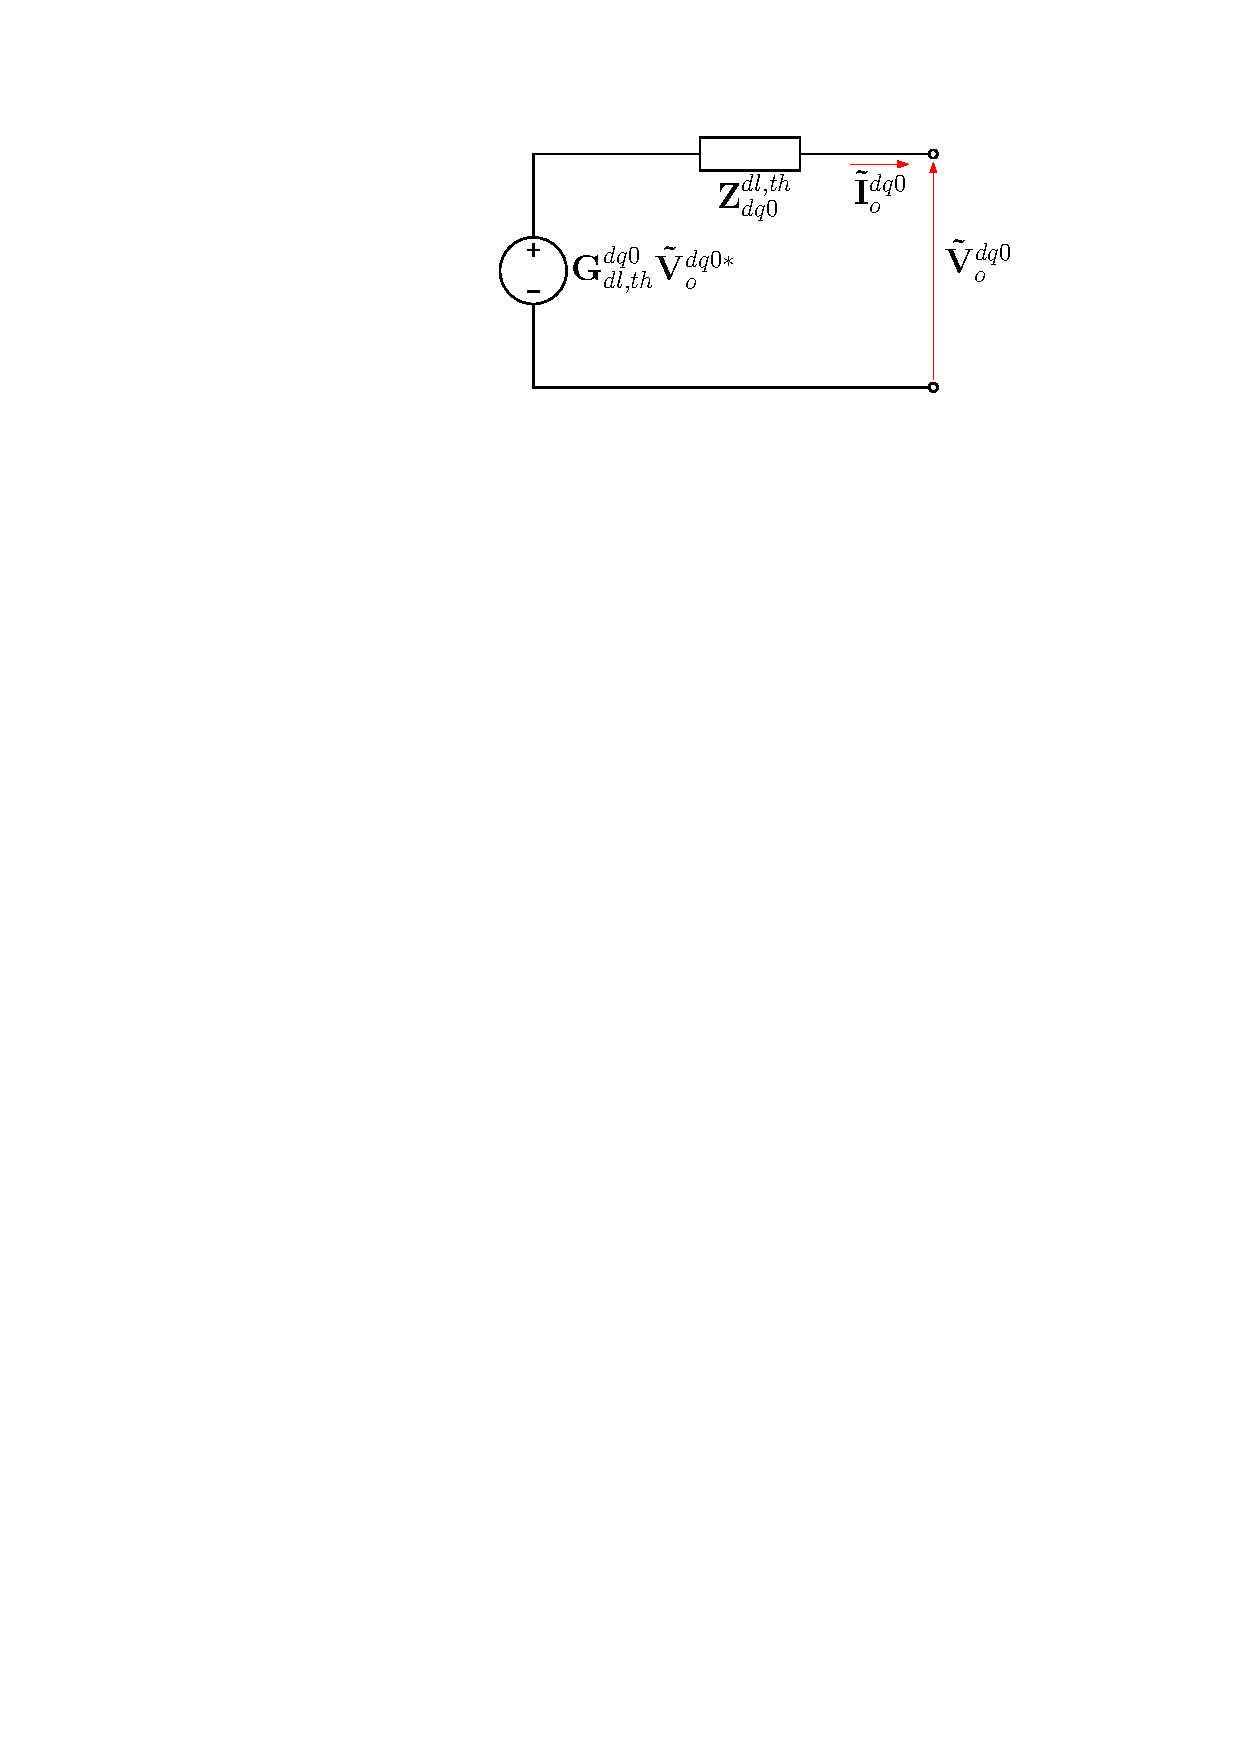
\includegraphics[width=0.9\linewidth]{./figuras/figuras_srf/Thevenin_SRF_VI}

\column{0.6\textwidth}


\begin{itemize}
	\item Impedância e ganho são matrizes $3 \times 3$\\[10pt]
	
	\item Representa a malha externa do MMC sob controle de malha dupla		
\end{itemize}

\end{columns}


\vspace*{0.5cm}

\begin{equation*}
\vetorgvcharzdldqL(s) = 
\left[
\vetorgicldqL(s) \vetorgvdq(s)
+\vetoryacdqL(s)
\right]^{-1} 
\end{equation*}


\begin{equation*}
\vetorgthdqL(s) = 
\left[ 
\mathbf{I} +
C_f \vetorgvcharzdldqL(s) \sdq 
\right]^{-1}
\vetorgvcharzdldqL(s) \vetorgicldqL(s) \vetorgvdq(s)
\end{equation*}

\begin{equation*}
\vetorzthdqL = 
\left[ 
\mathbf{I} +
C_f \vetorgvcharzdldqL(s) \sdq 
\right]^{-1}
\vetorgvcharzdldqL(s)
\end{equation*}

\end{frame}





%%%%%%%%%%%%%%%%%%%%%%%%%%%%%%%%%%%%%%%%%%%%%%%%%%%%%%%
%%%%%%%%%%%%%%%%%%%%%%%%%%%%%%%%%%%%%%%%%%%%%%%%%%%%%%%
%%%%%%%%%%%%%%%%%%%%%%%%%%%%%%%%%%%%%%%%%%%%%%%%%%%%%%%
\begin{frame}{Resposta em Frequência: $\vetorzthdqL$}

\begin{columns}

\column{0.5\textwidth}
\centering

Componente Própria

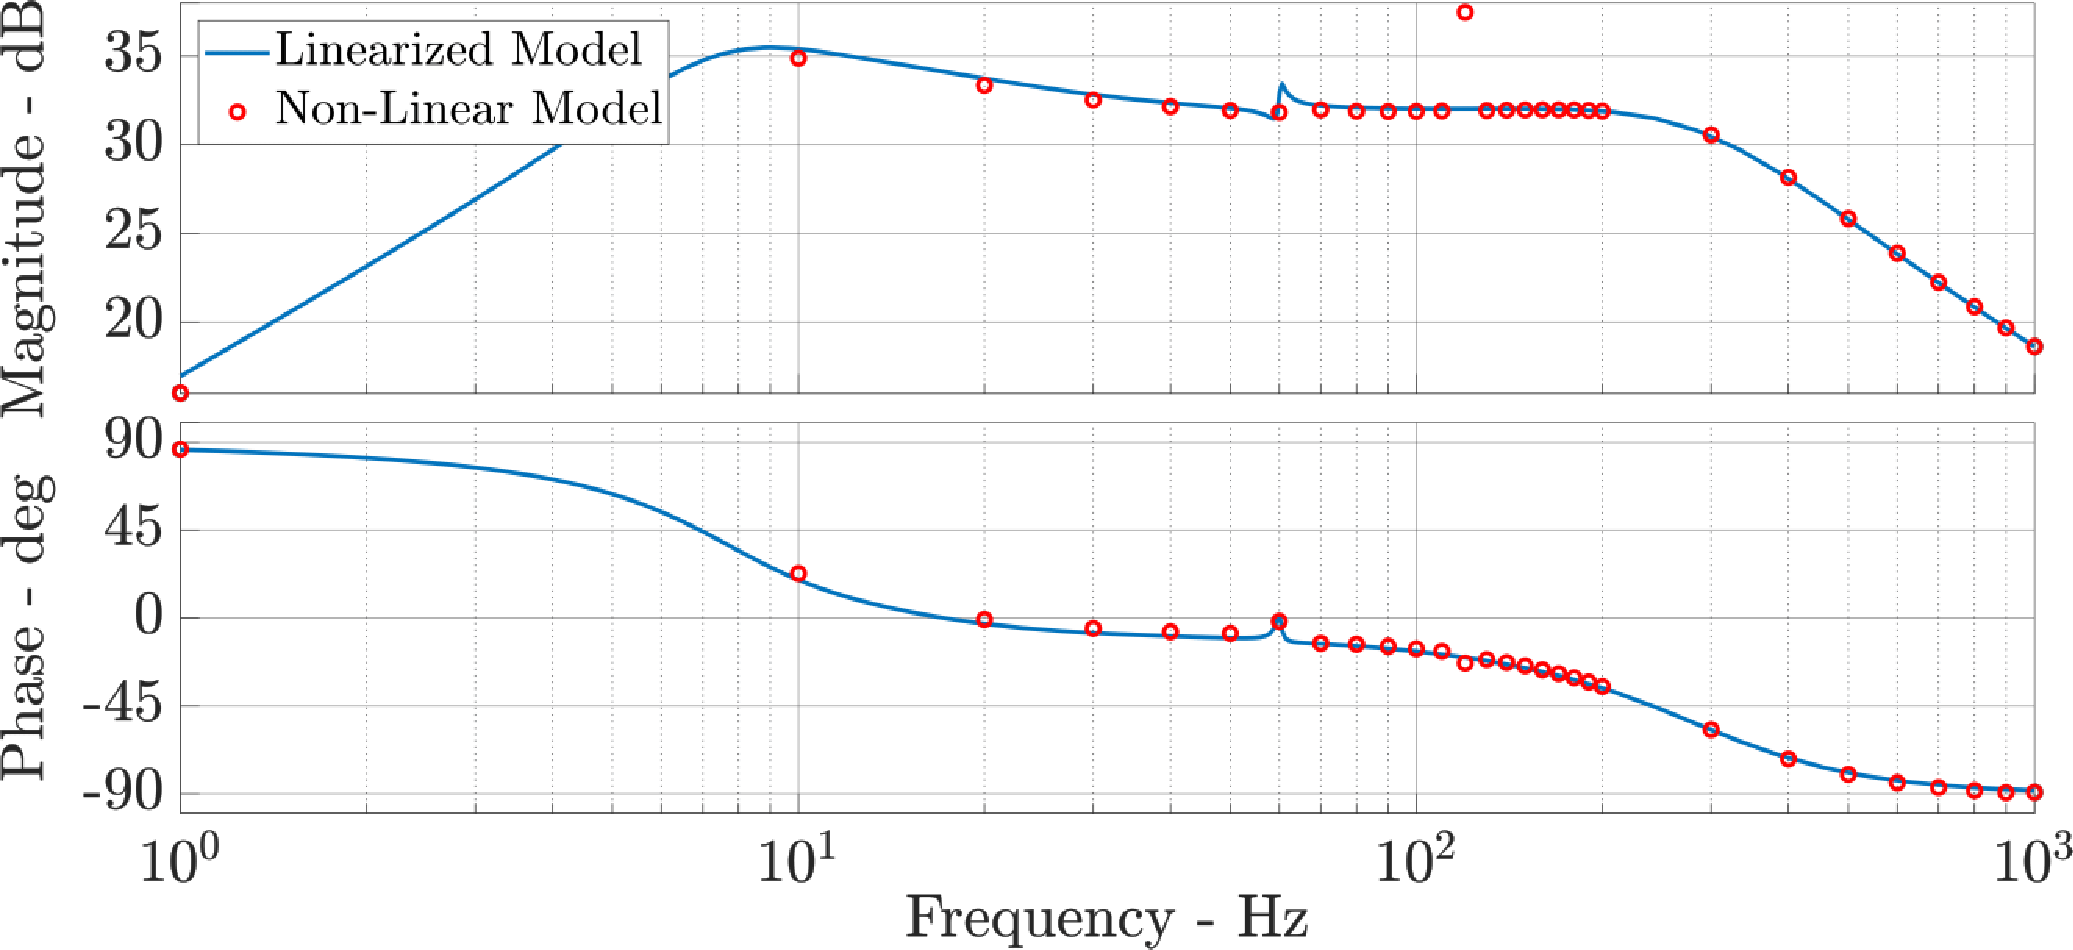
\includegraphics[width=0.88\linewidth]{./figuras/figuras_srf/bode_Z_th_dd}

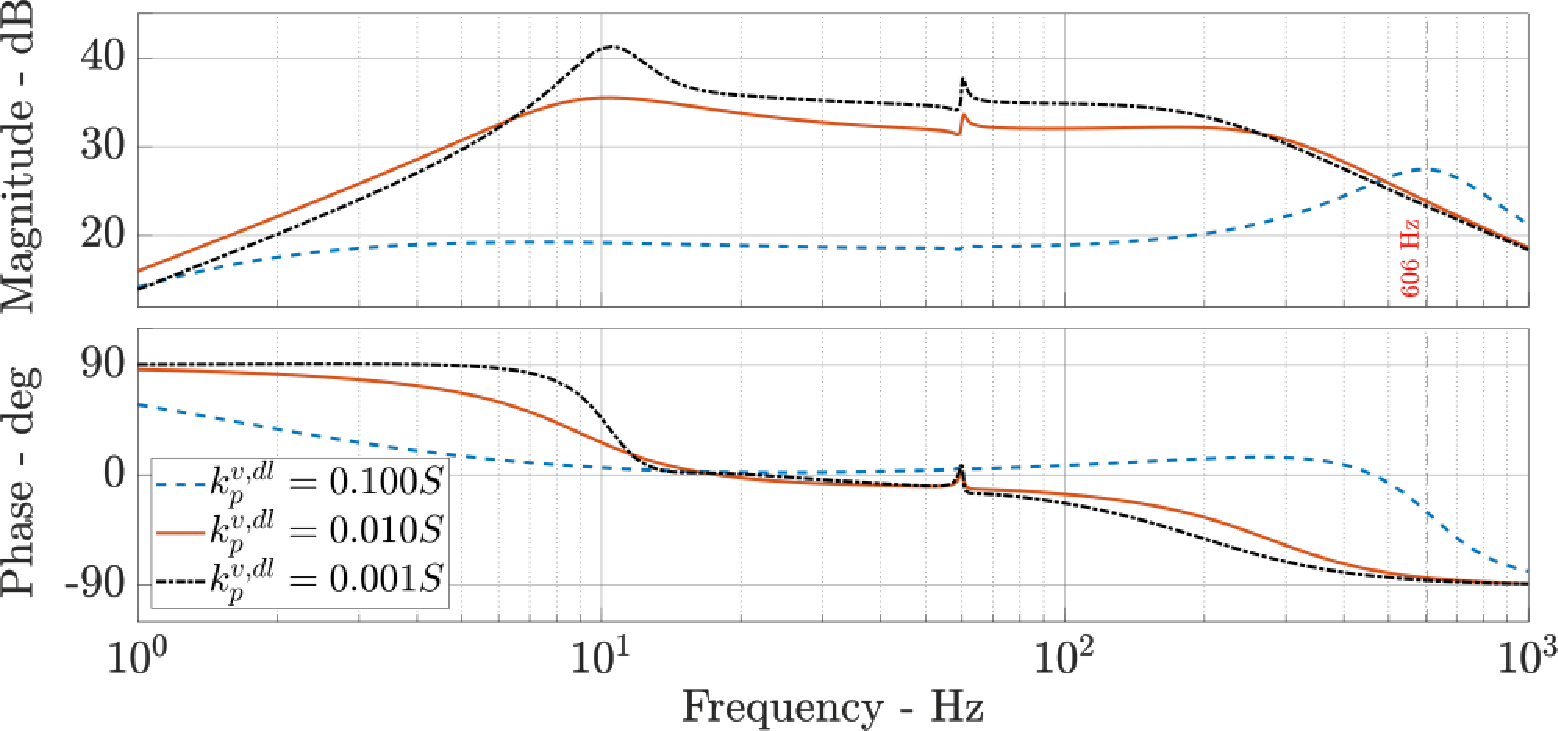
\includegraphics[width=0.88\linewidth]{./figuras/figuras_var_gain/bode_Zth_vdl_srf_dd_var_kpv}


\column{0.5\textwidth}
\centering


Componente Mútua

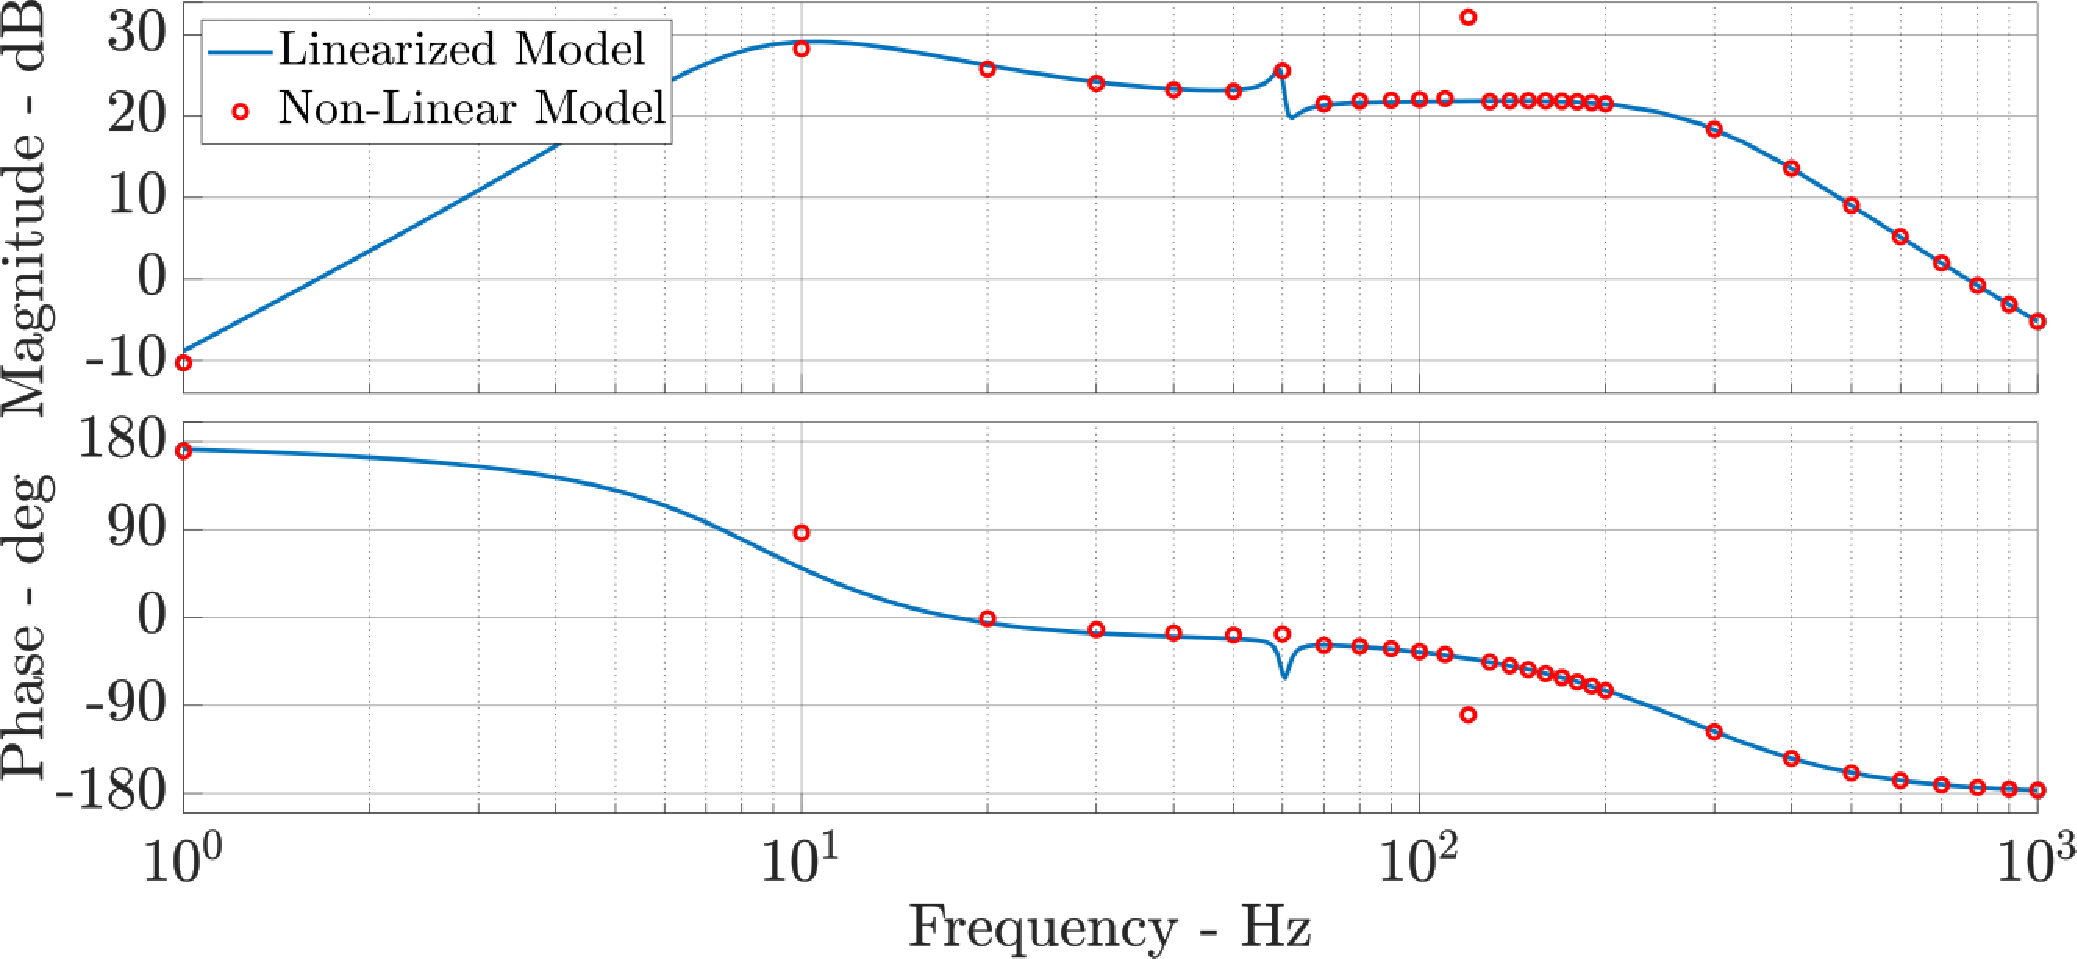
\includegraphics[width=0.88\linewidth]{./figuras/figuras_srf/bode_Z_th_dq}

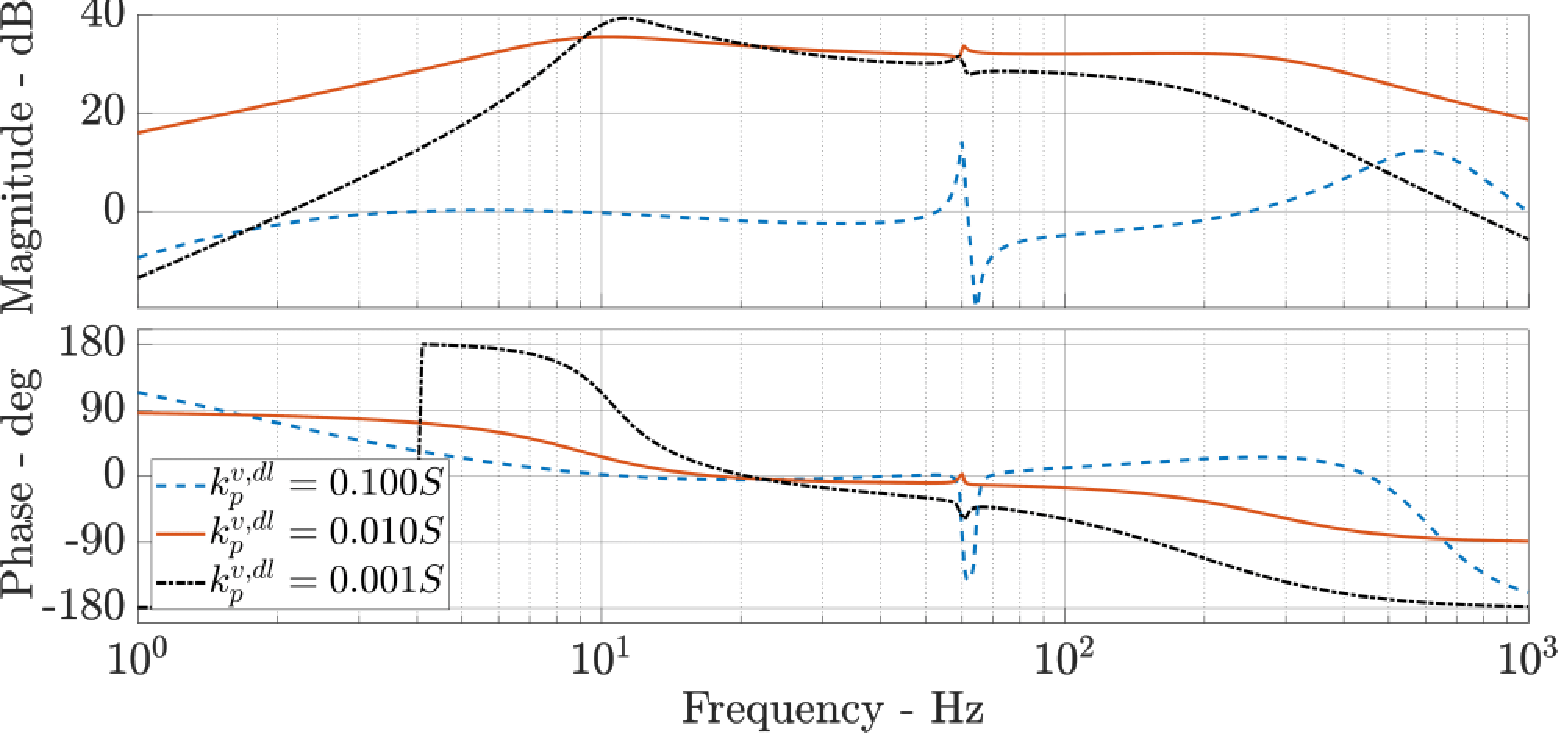
\includegraphics[width=0.88\linewidth]{./figuras/figuras_var_gain/bode_Zth_vdl_srf_dq_var_kpv}

\end{columns}



\end{frame}
